\section{GPU Implementation}
\label{sec:implementation}

This paper presents GPU implementations of the existing object
detection program using a popular computer vision technique
\cite{Niknejad12}.
Our contribution is distinguished from prior GPU implementations work
\cite{Chen11, Prisacariu09} in that we analyze the performance
characteristics of the object detection program to figure out what part
of the program should be accelerated using the GPU and our
implementations build on this analysis optimizing performance.

Note that this paper focuses on vehicle detection but the presented GPU
implementations and our technical contribution can be applied for other
object detection methods using HOG features and deformable models.

\subsection{Basic Understanding}
\label{sec:understanding}

In GPU programming, the GPU code and the input data typically need to be
copied from the host to the device memory before we launch a function,
\textit{a.k.a.}, a compute kernel, on the GPU.
The output data also needs to be copied back from the device to the host
memory so that the CPU can read them.
Hence the GPU-accelerated computation comes at the expense of the
offloading overhead.
Another shortcoming of the GPU is its relatively low operating frequency
as compared to the CPU due to the presence of a significant number of
compute cores.
These trade-offs must be addressed to benefit from GPU programming; it
is a complex undertaking for programmers to ascertain appropriate
computational blocks that can accelerate on the GPU.
Nonetheless this massively parallel computing architecture is becoming a
trend in the state of the art.
Given that GPUs outperform traditional multithreaded and multicore CPUs
in peak performance by an order of magnitude \cite{Kato13_2}, it is
worth exploring a more efficient way of GPU programming.
This paper provides a guideline of how to use GPUs in an efficient way
for vision-based object detection.

\subsection{Program Analysis}
\label{sec:analysis}

As aforementioned, the usage of the GPU depends highly on the program
structure.
If the program does not contain data-parallel compute-intensive blocks,
the GPU is not effective at all.
Therefore it is important to analyze the program prior to coding and
implementation.
The following is a summary of the program sequence for HOG-based object
detection using the deformable models.
The detailed procedure and algorithm description are presented in
\cite{Felzenszwalb10, Niknejad12}.

\begin{enumerate}
\item Load an input image.
\item Load the pre-defined object models.
\item Calculate HOG features for all resized variants of the input
      image, often referred to as a \textit{HOG pyramid}.
\item Calculate similarity scores for every set of the root/part filters
      and the resized HOG images.
\item Detect an object region based on a summation of the similarity
      scores.
\item Recognize an object based on the detection result.
\item Output the recognition result.
\end{enumerate}

\begin{figure}[t]
 \begin{center}
  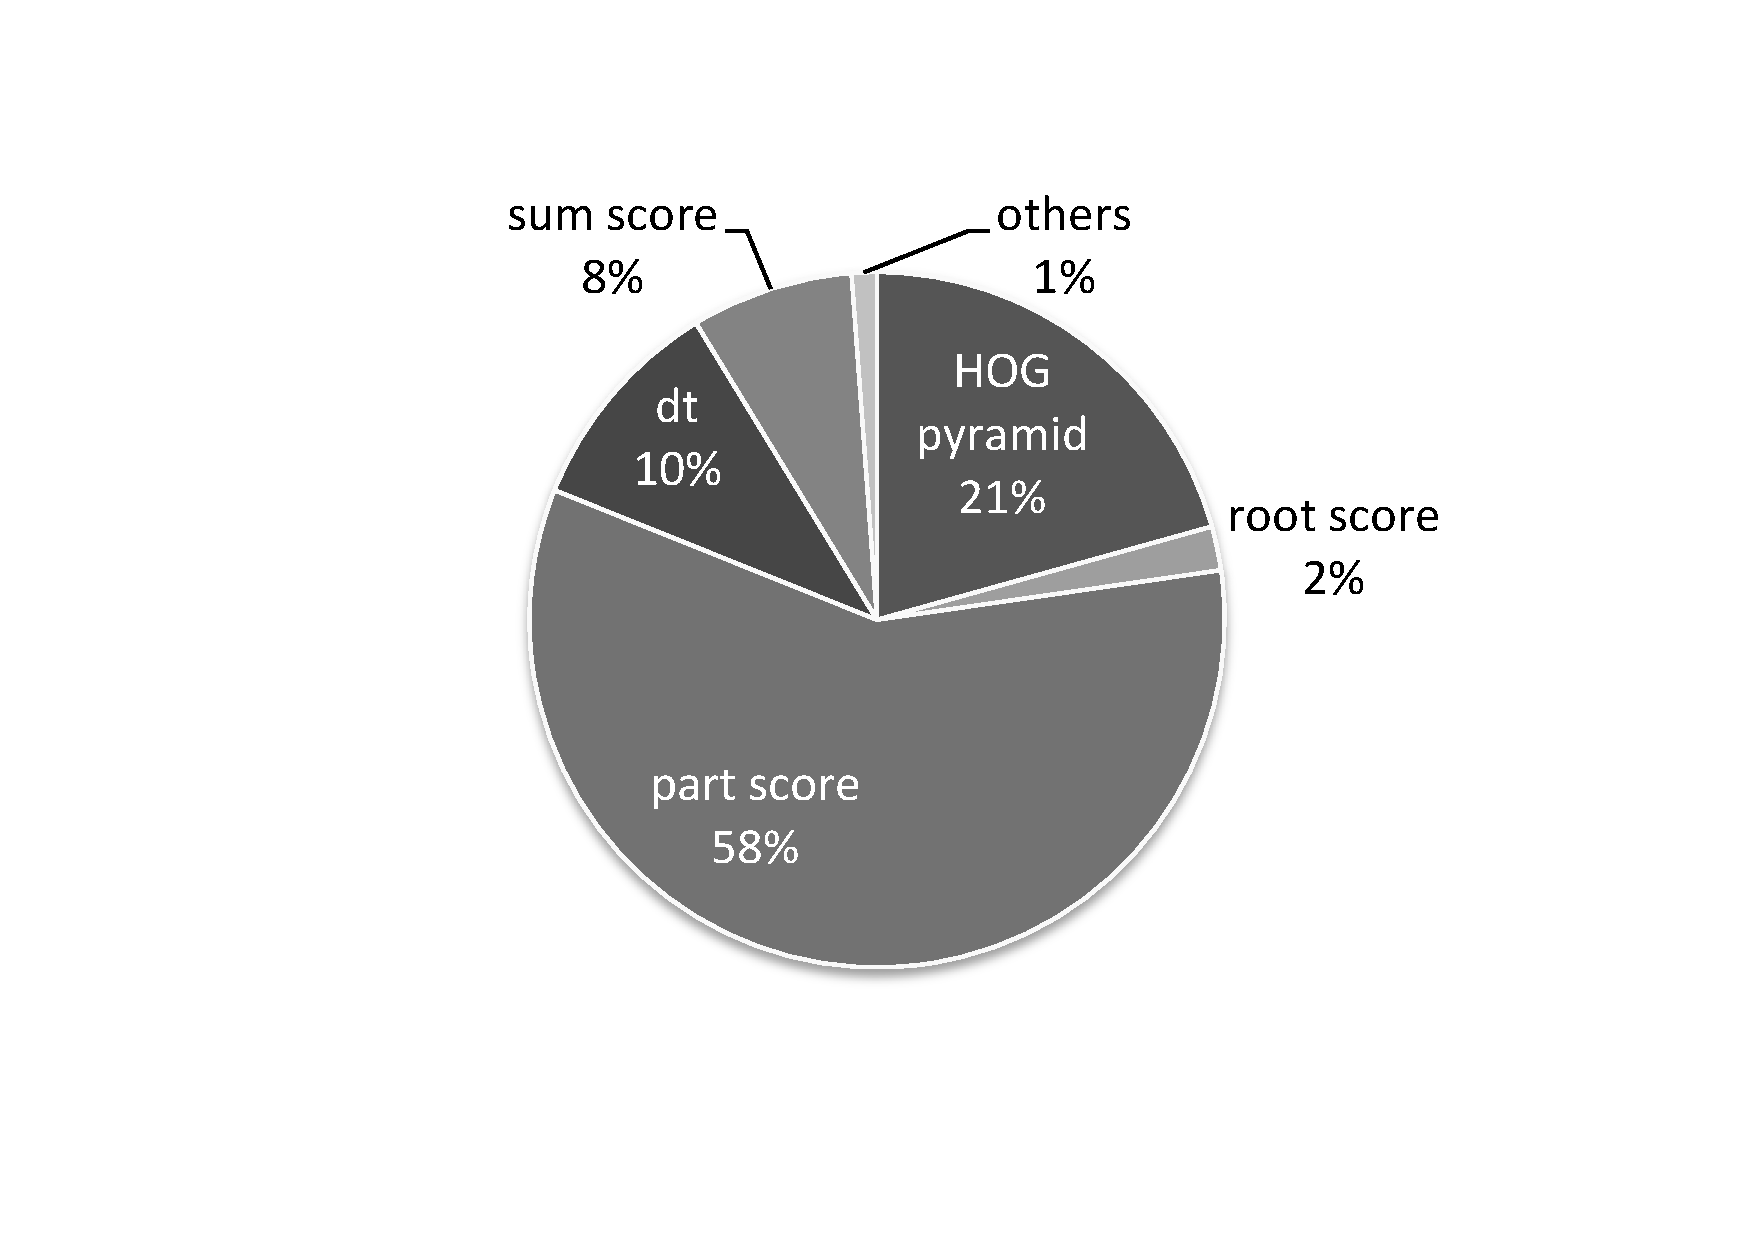
\includegraphics[width=\hsize]{fig/breakdown.pdf}\\
  \caption{The breakdown of computation times.}
  \label{fig:breakdown}
 \end{center}
\end{figure}

In order to identify computationally time-consuming blocks of the object
detection program, we conducted a preliminary measurement running the
original sequential code \cite{Niknejad12} on a standard Intel Core i7
2700K CPU.
The measurement approach is straightforward.
We find high-level \textit{for} loops (in case that the program is
written in the C-like language) by scanning the program structure and
make a timestamp for each loop.
The result of measurement is shown in Fig.~\ref{fig:breakdown}.
This breakdown of computation times provides us with a hint of how to
approach GPU implementations.
Specifically an obvious computational bottleneck appears in the
calculation of similarity scores againt the part filters, which
corresponds to partly ``Step 4)`` in the above program sequence.
This block dominates $58\%$ of the total time.
On the other hand, the calculation of HOG features corresponding ``Step
2)'' spends $21\%$ of the total time, while the detection and recognition
of the object, \textit{i.e.}, ``Step 5)'' and ``Step 6)'', contribute to
$10\%$ and $8\%$ of the total time respectively.

Our analysis conducted herein implies that even a simple time
measurement highlighting only the program structure without awareness of
the program context is helpful enough to understand computational
bottlenecks of the program.
In our case, it turned out that the most portion of the total time is
spent in the \textit{for} loops, which means that this program contains
a very high degree of parallelism and could be accelerated on the GPU.

\subsection{Implementation Approach}

\begin{figure}[t]
 \begin{center}
  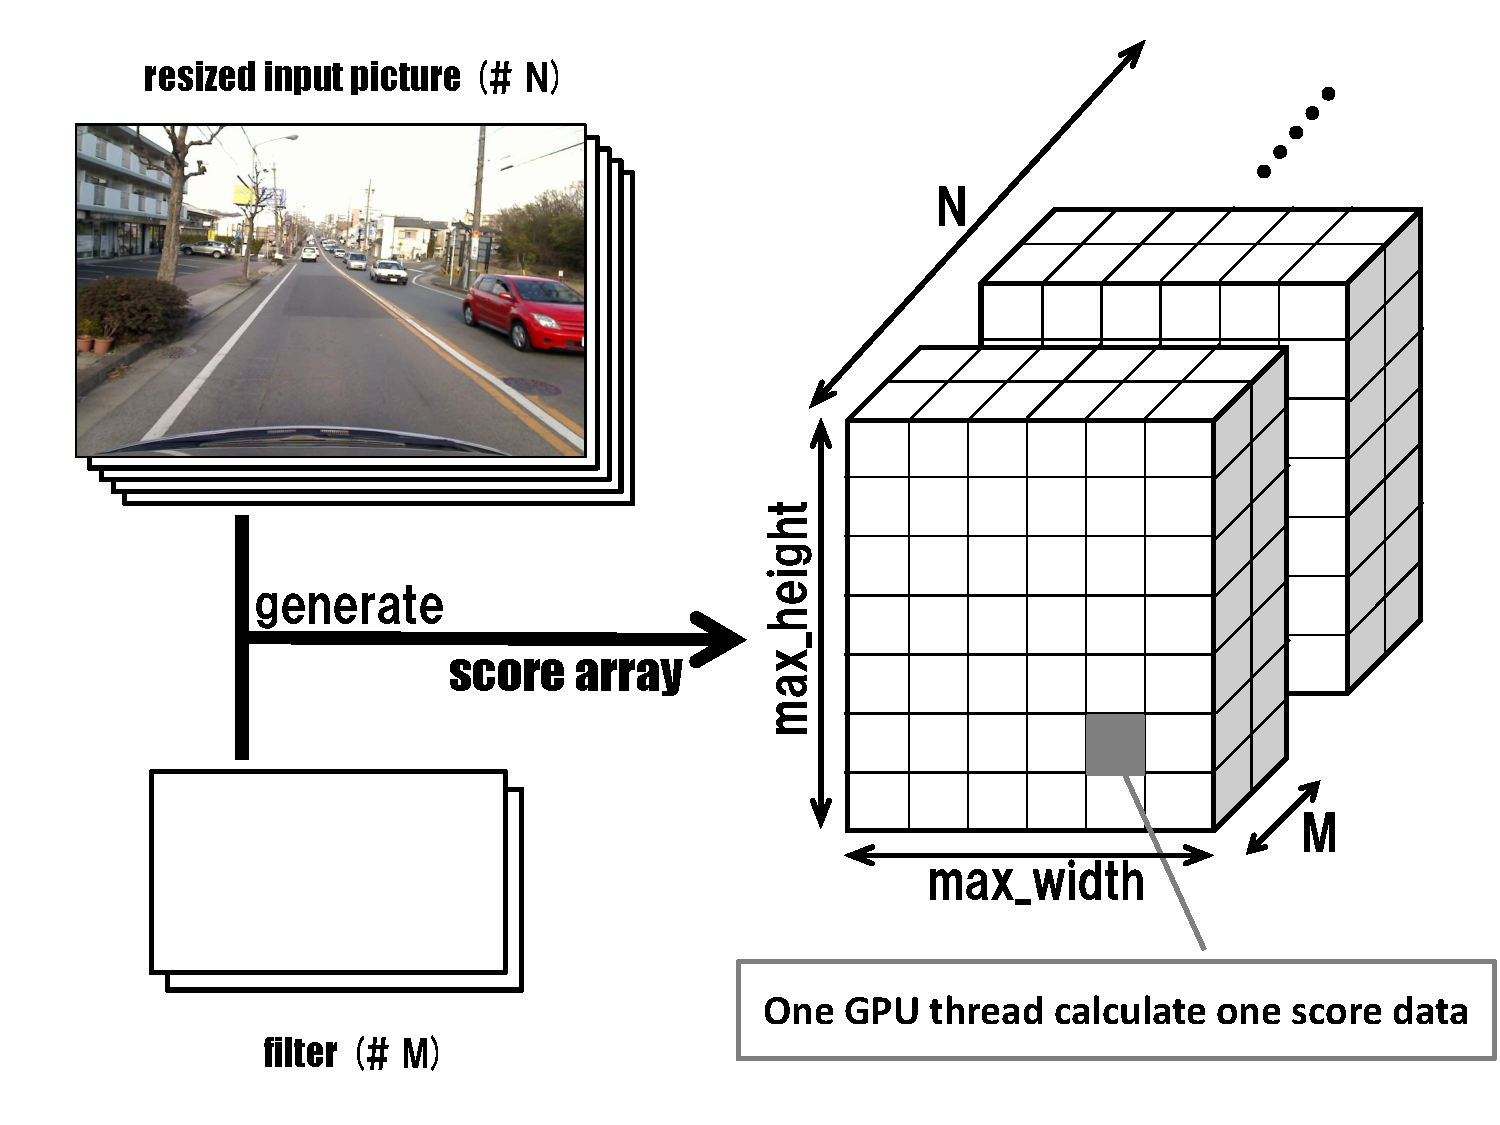
\includegraphics[width=\hsize]{fig/threads_shape.pdf}\\
  \caption{The number of compute threads and their block shape.}
  \label{fig:threads_shape}
 \end{center}
\end{figure}

\subsection{GPU Programming}